% =====================================================================
% Understanding GitHub: From Mental Models to Open Source Contribution
% Beamer presentation -- compile with pdflatex on Overleaf
% =====================================================================
\documentclass[10pt,aspectratio=169]{beamer}

% ---- Theme & colors ------------------------------------------------
\usetheme{metropolis}                 % If unavailable, try: \usetheme{Madrid}
\usecolortheme{default}
\metroset{sectionpage=none,subsectionpage=none}  % skip auto section pages

\definecolor{ghBg}{HTML}{0D1117}
\definecolor{ghAccent}{HTML}{2F81F7}
\definecolor{ghGreen}{HTML}{3FB950}
\definecolor{ghOrange}{HTML}{F78166}
\definecolor{ghMuted}{HTML}{8B949E}
\definecolor{codeBg}{HTML}{F6F8FA}

\setbeamercolor{frametitle}{bg=ghBg,fg=white}
\setbeamercolor{title separator}{fg=ghAccent}
\setbeamercolor{progress bar}{fg=ghAccent}
\setbeamercolor{alerted text}{fg=ghOrange}

% ---- Packages ------------------------------------------------------
\usepackage[utf8]{inputenc}
\usepackage[T1]{fontenc}
\usepackage{listings}
\usepackage{xcolor}
\usepackage{tikz}
\usepackage{booktabs}
\usepackage{array}
% fontawesome5 is available on Overleaf; fall back gracefully if not.
\IfFileExists{fontawesome5.sty}{\usepackage{fontawesome5}}{\providecommand{\faGithub}{[GH]}}
\usetikzlibrary{positioning,arrows.meta,shapes.geometric,calc}

% ---- Code listing style -------------------------------------------
\lstdefinestyle{bash}{
  basicstyle=\ttfamily\footnotesize,
  backgroundcolor=\color{codeBg},
  frame=single,
  framerule=0pt,
  rulecolor=\color{codeBg},
  xleftmargin=8pt,
  xrightmargin=8pt,
  aboveskip=4pt,
  belowskip=4pt,
  breaklines=true,
  showstringspaces=false,
  keywordstyle=\color{ghAccent}\bfseries,
  commentstyle=\color{ghMuted}\itshape,
  stringstyle=\color{ghGreen},
  language=bash,
  morekeywords={git,init,add,commit,push,pull,clone,branch,checkout,switch,
                merge,rebase,fetch,remote,log,diff,status,stash,reset,revert,
                cherry-pick,bisect,reflog,tag,restore},
}
\lstset{style=bash}

% ---- Title info ----------------------------------------------------
\title{Understanding GitHub}
\subtitle{From Mental Models to Open Source Contribution}
\author{A Self-Sufficient Reference}
\date{}

% =====================================================================
\begin{document}

% ---- Title (1) -----------------------------------------------------
\begin{frame}
  \titlepage
  \begin{center}
    \footnotesize\color{ghMuted}
    Git is the engine. GitHub is the city built around it.
  \end{center}
\end{frame}

% ---- Outline (2) ---------------------------------------------------
\begin{frame}{What this deck covers}
  \begin{columns}[T,onlytextwidth]
    \column{0.5\textwidth}
    \textbf{\color{ghAccent}Part I --- Foundations}
    \begin{itemize}
      \item Why version control exists
      \item Mental model: Git vs GitHub
      \item Core objects: commits, branches, refs
      \item Local workflow \& undoing mistakes
    \end{itemize}

    \vspace{0.5em}
    \textbf{\color{ghAccent}Part II --- Collaboration}
    \begin{itemize}
      \item Remotes, push/pull, origin
      \item Branching strategies
      \item Merge vs rebase, conflicts
      \item Pull requests \& reviews
    \end{itemize}

    \column{0.5\textwidth}
    \textbf{\color{ghAccent}Part III --- Open Source}
    \begin{itemize}
      \item Forks \& upstreams
      \item Issues, labels, CI/CD
      \item Maintainer etiquette
    \end{itemize}

    \vspace{0.5em}
    \textbf{\color{ghAccent}Part IV --- Advanced}
    \begin{itemize}
      \item History rewriting
      \item Recovery: reflog, bisect, stash
      \item Habits, resources, closing thoughts
    \end{itemize}
  \end{columns}
\end{frame}

% =====================================================================
% Part I --- Foundations
% =====================================================================

% ---- Why version control (3) ---------------------------------------
\begin{frame}{Why version control exists}
  \textbf{The problem:} files change over time, and you need to know
  \emph{what changed, when, why,} and \emph{by whom} --- and be able to
  go back.

  \vspace{0.6em}
  \textbf{Naive solutions fail at scale:}
  \begin{itemize}
    \item \texttt{final\_v2\_FINAL\_real.py} --- no real history
    \item Dropbox / Drive --- overwrites, no branching, no review
    \item Email attachments --- no merge, no provenance
  \end{itemize}

  \vspace{0.6em}
  \textbf{Git's answer:} a \alert{content-addressed snapshot store}
  with a graph of changes you can branch, merge, inspect, and rewind.

  \vspace{0.8em}
  \begin{center}
    \footnotesize\color{ghMuted}
    For research: every experiment becomes a checkpoint.
    For engineering: every change becomes reviewable.
  \end{center}
\end{frame}

% ---- Mental model (4) ----------------------------------------------
\begin{frame}{Mental model: Git vs GitHub}
  \begin{center}
  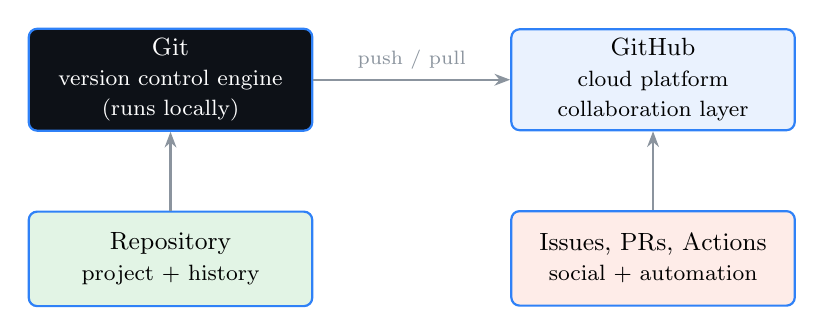
\begin{tikzpicture}[
      node distance=1.4cm,
      box/.style={rectangle, rounded corners=3pt, draw=ghAccent, thick,
                  minimum width=3.6cm, minimum height=1.2cm, align=center,
                  font=\small},
      arrow/.style={-{Stealth[length=2mm]}, thick, ghMuted}
    ]
    \node[box, fill=ghBg, text=white] (git) {Git\\\footnotesize version control engine\\\footnotesize (runs locally)};
    \node[box, right=2.5cm of git, fill=ghAccent!10] (gh) {GitHub\\\footnotesize cloud platform\\\footnotesize collaboration layer};
    \node[box, below=1cm of git, fill=ghGreen!15] (repo) {Repository\\\footnotesize project + history};
    \node[box, below=1cm of gh, fill=ghOrange!15] (social) {Issues, PRs, Actions\\\footnotesize social + automation};

    \draw[arrow] (git) -- node[above,font=\scriptsize]{push / pull} (gh);
    \draw[arrow] (repo) -- (git);
    \draw[arrow] (social) -- (gh);
  \end{tikzpicture}
  \end{center}

  \vspace{0.4em}
  \begin{itemize}
    \item \textbf{Git} works without an internet connection.
    \item \textbf{GitHub} is one of several hosts (others: GitLab, Codeberg, Bitbucket).
    \item You can use Git without GitHub. You cannot use GitHub without Git.
  \end{itemize}
\end{frame}

% ---- Core objects (5) ----------------------------------------------
\begin{frame}{Core objects you should picture in your head}
  \begin{columns}[T]
    \column{0.5\textwidth}
    \textbf{\color{ghAccent}Commit}\\
    A snapshot of all tracked files + a message + a parent pointer.
    Identified by a SHA hash (\texttt{a3f8c1d...}).

    \vspace{0.6em}
    \textbf{\color{ghAccent}Branch}\\
    A movable pointer to a commit. Cheap to create
    (\texttt{git branch} is just writing a 40-char hash to a file).

    \vspace{0.6em}
    \textbf{\color{ghAccent}HEAD}\\
    A pointer to ``where you are right now'' --- usually to a branch,
    sometimes directly to a commit (\emph{detached HEAD}).

    \column{0.5\textwidth}
    \textbf{\color{ghAccent}Working tree}\\
    The actual files on disk you edit.

    \vspace{0.6em}
    \textbf{\color{ghAccent}Staging area (index)}\\
    A drafting area where you pick \emph{which} changes go into the next commit.

    \vspace{0.6em}
    \textbf{\color{ghAccent}Repository}\\
    The \texttt{.git/} folder --- the database of every object and ref.
  \end{columns}

  \vspace{0.8em}
  \begin{center}
    \footnotesize\color{ghMuted}
    Three zones: \textbf{working tree} $\to$ \textbf{staging} $\to$ \textbf{repository}.
  \end{center}
\end{frame}

% ---- Local workflow + undoing (6) ----------------------------------
\begin{frame}[fragile]{Local workflow \& undoing mistakes}
\begin{lstlisting}
git init                    # start a new repo
git status                  # see what's changed
git add path/to/file        # stage a specific file
git add .                   # stage everything in current dir
git commit -m "Fix M-value transform for zero-variance CpGs"
git log --oneline --graph --decorate
git diff                    # see unstaged changes
\end{lstlisting}

  \textbf{Safety net --- undoing things:}
\begin{lstlisting}
git restore <file>              # discard working-tree changes (destructive)
git restore --staged <file>     # unstage but keep edits
git commit --amend              # fix the last commit (msg or content)
git reset --soft HEAD~1         # undo last commit, KEEP changes
git reset --hard HEAD~1         # undo last commit, THROW AWAY changes (danger)
git revert <sha>                # NEW commit that reverses an old one (safe for shared history)
\end{lstlisting}
  \alert{Rule:} \texttt{reset --hard} and force-push are the only real ways to lose work. Everything else is recoverable via \texttt{reflog}.
\end{frame}

% =====================================================================
% Part II --- Collaboration
% =====================================================================

% ---- Remotes (7) ---------------------------------------------------
\begin{frame}[fragile]{Remotes: connecting your local repo to GitHub}
\begin{lstlisting}
# Clone an existing repo (most common starting point)
git clone https://github.com/user/repo.git

# Or: link a local repo to a new GitHub remote
git remote add origin https://github.com/user/repo.git
git push -u origin main          # -u sets upstream tracking

# See your remotes
git remote -v

# Sync
git push                          # send local commits up
git pull                          # fetch + merge from remote
git fetch                         # fetch only, don't merge
\end{lstlisting}

  \textbf{Terminology:}
  \begin{itemize}
    \item \texttt{origin} --- conventional name for \emph{your} primary remote
    \item \texttt{upstream} --- conventional name for the \emph{original} repo you forked from
    \item \texttt{main} (or \texttt{master}) --- the default branch name
  \end{itemize}
\end{frame}

% ---- Branching (8) -------------------------------------------------
\begin{frame}[fragile]{Branching: parallel timelines for safe experimentation}
\begin{lstlisting}
git switch -c feature/wkde-scoring   # create + switch (modern)
git checkout -b feature/wkde-scoring # equivalent (older)
git branch                            # list local
git branch -a                         # local + remote
git switch main                       # change branch
git branch -d feature/wkde-scoring    # delete (after merge)
\end{lstlisting}

  \vspace{0.4em}
  \textbf{Why branches matter for research:}
  \begin{itemize}
    \item One branch per experiment / hypothesis / feature
    \item \texttt{main} stays clean and reproducible
    \item Failed experiments don't pollute history --- just don't merge them
    \item Cheap and disposable: a branch is a 40-character pointer, not a copy
  \end{itemize}
\end{frame}

% ---- Merge vs rebase (9) -------------------------------------------
\begin{frame}{Merge vs rebase: two ways to combine branches}
  \begin{columns}[T]
    \column{0.5\textwidth}
    \textbf{\color{ghAccent}Merge}\\[0.3em]
    Creates a new ``merge commit'' that ties two histories together.
    \begin{itemize}
      \item \textbf{Pros:} preserves true history, non-destructive
      \item \textbf{Cons:} graph can look tangled
      \item \textbf{Use for:} shared branches, public history
    \end{itemize}
    \begin{center}
      \scriptsize\ttfamily
      A---B---C---M\\
      ~~~~~~~~\textbackslash~~~~~/\\
      ~~~~~~~~~D---E
    \end{center}

    \column{0.5\textwidth}
    \textbf{\color{ghAccent}Rebase}\\[0.3em]
    Re-applies your commits on top of another branch, rewriting history.
    \begin{itemize}
      \item \textbf{Pros:} linear, clean history
      \item \textbf{Cons:} rewrites SHAs --- dangerous on shared branches
      \item \textbf{Use for:} cleaning up \emph{your own} feature branch before PR
    \end{itemize}
    \begin{center}
      \scriptsize\ttfamily
      A---B---C---D'---E'
    \end{center}
  \end{columns}

  \vspace{0.6em}
  \begin{center}
    \alert{Golden rule:} never rebase commits that others have already pulled.
  \end{center}
\end{frame}

% ---- Merge conflicts (10) ------------------------------------------
\begin{frame}[fragile]{Merge conflicts: not a bug, a conversation}
  A conflict happens when two branches change the \emph{same lines} of the
  same file. Git pauses and asks you to decide.

\begin{lstlisting}
<<<<<<< HEAD
result = compute_mvalue(beta, epsilon=1e-6)
=======
result = compute_mvalue(beta, eps=1e-5)
>>>>>>> feature/wkde-scoring
\end{lstlisting}

  \textbf{Resolve by:}
  \begin{enumerate}
    \item Editing the file --- pick one side, combine, or rewrite
    \item Remove the \texttt{<<<<}, \texttt{====}, \texttt{>>>>} markers
    \item \texttt{git add <file>} to mark it resolved
    \item \texttt{git commit} (for merge) or \texttt{git rebase --continue} (for rebase)
  \end{enumerate}

  \vspace{0.4em}
  \begin{center}
    \footnotesize\color{ghMuted}
    Practice tip: deliberately create a conflict in a throwaway repo. Twice. You'll never fear them again.
  \end{center}
\end{frame}

% ---- Pull requests (11) --------------------------------------------
\begin{frame}{Pull requests: the scientific peer review of code}
  A \textbf{pull request} (PR) is a proposal: ``please merge my branch into yours,
  here's what I changed and why.''

  \vspace{0.5em}
  \textbf{Anatomy of a good PR:}
  \begin{itemize}
    \item \textbf{Title} --- imperative mood: \emph{``Add HSIC test for continuous variables''}
    \item \textbf{Description} --- what, why, how to test, related issue
    \item \textbf{Small scope} --- one logical change; reviewers can't review 2000-line PRs well
    \item \textbf{Tests} --- if the project has them, add or update them
    \item \textbf{Linked issue} --- \texttt{Closes \#42}
  \end{itemize}

  \vspace{0.5em}
  \textbf{The review loop:}
  reviewer comments $\to$ you push new commits to the same branch $\to$
  PR updates automatically $\to$ approve $\to$ merge.

  \vspace{0.5em}
  \begin{center}
    \footnotesize\color{ghMuted}
    Think of a PR as a manuscript submission. The reviewers want it to land.
  \end{center}
\end{frame}

% =====================================================================
% Part III --- Open Source
% =====================================================================

% ---- Fork workflow (12) --------------------------------------------
\begin{frame}[fragile]{The fork + upstream workflow}
  You usually can't push directly to someone else's repo. Instead:

  \begin{enumerate}
    \item \textbf{Fork} their repo on GitHub (creates your copy)
    \item \textbf{Clone} your fork locally
    \item Add the original as \texttt{upstream}
    \item Create a feature branch, commit, push to your fork
    \item Open a PR from your fork $\to$ their repo
  \end{enumerate}

\begin{lstlisting}
git clone https://github.com/you/their-repo.git
cd their-repo
git remote add upstream https://github.com/them/their-repo.git

# Keep your fork in sync with upstream
git fetch upstream
git switch main
git rebase upstream/main
git push origin main
\end{lstlisting}
\end{frame}

% ---- Issues + CI/CD combined (13) ----------------------------------
\begin{frame}{The social \& automation layer: issues, labels, CI/CD}
  \begin{columns}[T]
    \column{0.5\textwidth}
    \textbf{\color{ghAccent}Issues}\\
    Bug reports, feature requests, questions. \emph{Always search before opening one.}

    \vspace{0.4em}
    \textbf{\color{ghAccent}Labels to look for}\\
    \texttt{good first issue}, \texttt{help wanted}, \texttt{bug},
    \texttt{documentation}. Your entry points.

    \vspace{0.4em}
    \textbf{\color{ghAccent}Discussions \& templates}\\
    Open-ended Q\&A; fill out issue/PR templates properly --- it's the
    difference between attention and an immediate close.

    \column{0.5\textwidth}
    \textbf{\color{ghAccent}CI = Continuous Integration}\\
    Every push runs automated checks: tests, linters, type-checkers,
    builds. Configured in \texttt{.github/workflows/*.yml}.

    \vspace{0.4em}
    \textbf{\color{ghAccent}CD = Continuous Deployment}\\
    Successful builds can auto-publish releases, deploy docs, push packages.

    \vspace{0.4em}
    \textbf{\color{ghAccent}Why this matters for your PR}\\
    Status checks must be green. \texttt{pytest}, \texttt{ruff},
    \texttt{mypy}, \texttt{black} commonly enforced. Maintainers will
    not merge red builds.
  \end{columns}
\end{frame}

% ---- Etiquette (14) ------------------------------------------------
\begin{frame}{Etiquette: how to actually get merged}
  \textbf{Before opening a PR:}
  \begin{itemize}
    \item Read \texttt{CONTRIBUTING.md} --- it tells you the rules of the house
    \item Check \texttt{CODE\_OF\_CONDUCT.md}
    \item Search existing issues and PRs --- yours might be a duplicate
    \item Open an issue first for non-trivial changes; get buy-in before coding
  \end{itemize}

  \vspace{0.4em}
  \textbf{In your PR:}
  \begin{itemize}
    \item Be patient. Maintainers volunteer their time.
    \item Respond to review comments; don't be defensive
    \item Squash noisy commits if asked
    \item Update your branch when conflicts arise --- don't expect them to do it
  \end{itemize}

  \vspace{0.4em}
  \textbf{After your PR:}
  \begin{itemize}
    \item Stick around. The first contribution is the hardest;
          the second is easy. The tenth makes you a regular.
  \end{itemize}
\end{frame}

% =====================================================================
% Part IV --- Advanced
% =====================================================================

% ---- Interactive rebase (15) ---------------------------------------
\begin{frame}[fragile]{Interactive rebase: curating your own history}
\begin{lstlisting}
git rebase -i HEAD~5    # edit the last 5 commits
\end{lstlisting}

  Opens an editor with a list:
\begin{lstlisting}
pick   a1b2c3d Add WKDE skeleton
pick   d4e5f6g typo
pick   g7h8i9j Add tests
pick   j1k2l3m wip
pick   m4n5o6p Finalize WKDE scoring
\end{lstlisting}

  Change \texttt{pick} to:
  \begin{itemize}
    \item \texttt{reword} --- edit the commit message
    \item \texttt{squash} (\texttt{s}) --- merge into previous commit
    \item \texttt{fixup} (\texttt{f}) --- like squash but discard message
    \item \texttt{drop} (\texttt{d}) --- remove the commit entirely
    \item reorder lines to reorder commits
  \end{itemize}

  \vspace{0.3em}
  \alert{Only do this on commits you haven't pushed, or on a personal feature branch.}
\end{frame}

% ---- Advanced toolbox (16) -----------------------------------------
\begin{frame}[fragile]{The advanced toolbox: stash, cherry-pick, reflog, bisect, tag}
\begin{lstlisting}
# Temporarily shelve uncommitted changes (e.g. to switch branch)
git stash; git stash list; git stash pop

# Apply a single commit from another branch onto yours
git cherry-pick <sha>

# Reflog: a log of every HEAD movement -- your real safety net
git reflog
git checkout <sha>; git switch -c recovered-branch

# Bisect: binary-search history to find which commit broke something
git bisect start
git bisect bad                    # current commit is broken
git bisect good v1.0.0            # this old tag worked
# git checks out the midpoint; you test, then mark good/bad. Repeat.
git bisect reset

# Tag an immutable release point
git tag -a v1.0.0 -m "First release"
git push origin v1.0.0
\end{lstlisting}
\end{frame}

% ---- Concepts table (17) -------------------------------------------
\begin{frame}{High-level concepts worth internalizing}
  \begin{center}
  \renewcommand{\arraystretch}{1.25}
  \begin{tabular}{>{\color{ghAccent}\bfseries}l p{8.5cm}}
    \toprule
    Concept & Why it matters \\
    \midrule
    Version control   & Reproducibility of experiments and results \\
    Branching         & Safe parallel experimentation \\
    Commits           & Research checkpoints with provenance \\
    Pull requests     & Code review as scientific peer review \\
    CI/CD             & Automated validation of every change \\
    Forks             & Independent lines of work without permission \\
    Tags / releases   & Citable, immutable snapshots \\
    Git history       & A readable record of how knowledge evolved \\
    \bottomrule
  \end{tabular}
  \end{center}

  \vspace{0.6em}
  \begin{center}
    \footnotesize\color{ghMuted}
    Git is, deep down, a tool for thinking carefully about how change happens over time.
  \end{center}
\end{frame}

% ---- Habits (18) ---------------------------------------------------
\begin{frame}{Habits that separate beginners from research engineers}
  \begin{columns}[T]
    \column{0.5\textwidth}
    \textbf{\color{ghGreen}Do}
    \begin{itemize}
      \item Commit early, commit often
      \item Write messages your future self will thank you for
      \item One branch per logical change
      \item Pull / rebase before starting work
      \item Use \texttt{.gitignore} from day one
      \item Tag releases of papers / experiments
      \item Read the diff before you commit
    \end{itemize}

    \column{0.5\textwidth}
    \textbf{\color{ghOrange}Don't}
    \begin{itemize}
      \item Commit secrets (keys, tokens) --- they live in history forever
      \item Commit huge binary files --- use Git LFS or DVC
      \item Force-push to shared branches
      \item Use \texttt{git add .} blindly
      \item Treat \texttt{main} as your scratchpad
      \item Write messages like \texttt{"fix"} or \texttt{"update"}
      \item Ignore CI failures
    \end{itemize}
  \end{columns}
\end{frame}

% ---- Plan + resources (19) -----------------------------------------
\begin{frame}{30-day plan \& where to read next}
  \begin{center}
  \renewcommand{\arraystretch}{1.2}
  \begin{tabular}{>{\color{ghAccent}\bfseries}l p{9cm}}
    \toprule
    Week & Focus \\
    \midrule
    1 & Basic Git: \texttt{init, add, commit, log, diff, status}. Version your notes daily. \\
    2 & GitHub: push/pull, README, \texttt{.gitignore}. Build a portfolio repo. \\
    3 & Branching, merges, deliberate conflicts, your first PR. \\
    4 & Open source: fork, sync upstream, contribute one small fix. \\
    \bottomrule
  \end{tabular}
  \end{center}

  \vspace{0.5em}
  \textbf{References}: \emph{Pro Git} book (\texttt{git-scm.com/book}); official docs (\texttt{git-scm.com/doc}); GitHub Skills (\texttt{skills.github.com}).

  \vspace{0.3em}
  \textbf{Entry points}: \emph{First Contributions} (\texttt{firstcontributions.github.io}); \emph{Awesome for Beginners}; any repo's \texttt{good first issue} label.

  \vspace{0.3em}
  \textbf{Repos worth reading}: \texttt{pgmpy/pgmpy} (relevant to your causal work), \texttt{scikit-learn/scikit-learn}, \texttt{pytorch/pytorch}.
\end{frame}

% ---- Closing (20) --------------------------------------------------
\begin{frame}{One closing insight}
  Most people use only:
  \begin{center}
    \texttt{git add} \quad \texttt{git commit} \quad \texttt{git push} \quad \texttt{git pull}
  \end{center}

  \vspace{0.6em}
  Advanced users think in:
  \begin{itemize}
    \item history rewriting and curation
    \item collaboration systems and review culture
    \item reproducibility of experiments
    \item workflow design and automation
    \item safety nets for experimentation
  \end{itemize}

  \vspace{0.8em}
  \begin{center}
    \large\color{ghAccent}
    Git is not a tool you finish learning.\\
    It's a medium you keep thinking in.
  \end{center}

  \vspace{0.4em}
  \begin{center}
    \footnotesize\color{ghMuted}
    \faGithub\ \ Happy committing.
  \end{center}
\end{frame}

\end{document}